
%\fitter\ is a unique QCD fit platform that provides many options to the user to perform a quantitative assessment of impact level for a new data or new theoretical prediction. The quest on nailing down the uncertainties on PDFs have lead, on one hand, to highly precise measurements that are in need of careful handling of all provided sources of uncertainties, and on the other hand to numerous software packages that provide higher order calculations in QCD to match the precision of data.



There are a considerable number of choices available when performing a QCD fit analysis which require careful investigation (i.e. functional parametrisation form, heavy quark masses, alternative theoretical calculations, method of minimisation, interpretation of uncertainties etc.).
%
 It is desirable to be able to discriminate or quantify the effect of the chosen ansatz, ideally within a common framework, and 
\fitter\ is optimally designed for such tests.
%
The methodology employed by \fitter\  relies on a flexible and modular
framework that allows for independent integration of the state-of-the-art techniques, either related to the inclusion of a new theoretical calculation, or to new approaches to treat uncertainties. 
%

In this section we briefly describe the available options in \fitter\ ranging from the functional form used to parametrise PDFs and the choice of the form of the $\chi^2$ function, to different methods to assess the experimental uncertainties on extracted PDFs.

%list various types of functional forms used to parametrise PDFs, different definitions for  $\chi^2$ evaluation in extracting the PDF parameters which account for correlated and uncorrelated sources of experimental (or theoretical) uncertainties available in \fitter. 
In addition, as an alternative approach to a complete QCD fit,  the Bayesian reweighting
method, which is also available in the \fitter, is described in this section. 



\subsection{Functional Forms for PDF parametrisation}
The PDFs are parametrised at a starting scale which is chosen by the user. Various functional forms can be tested using free parameters to be extracted from the fit:
\begin{description}
\item \bf {Standard Polynomials:} \rm
The term standard is understood to refer to a simple polynomial 
that interpolates between the low and high $x$ regions:
\begin{equation}
 xf(x) = A x^{B} (1-x)^{C} P_i(x),
\label{eqn:pdf_std}
\end{equation}
Standard forms are commonly used by PDF groups.
The parametrised PDFs at HERA are the valence distributions
$xu_v$ and $xd_v$, the gluon distribution $xg$, and the $u$-type and $d$-type sea 
$x\bar{U}$, $x\bar{D}$, where $x\bar{U} = x\bar{u}$, 
$x\bar{D} = x\bar{d} +x\bar{s}$ at the starting scale chosen below the charm mass threshold. 
The $P_i(x)$ for the HERAPDF~\cite{h1zeus:2009wt} style takes the simple Regge-inspired form  
$(1 + \epsilon \sqrt{x} + D x + E x^2)$
with additional constraints relating to the flavour decomposition of the 
light sea. 
For the CTEQ style, $P_i(x)$ takes the form $e^{a_3x} (1 + e^{a_4} x + e^{a_5} x^2)$.
QCD number and momentum sum-rules are used to determine the normalisations $A$ for the valence and gluon distributions. 
The sum-rules can be evaluated analytically.

\item \bf {Log-Normal Distributions:} \rm
A bi-log-normal distribution to parametrise the $x$ dependence of the PDFs is 
also available in \fitter.
%parton distribution function of the proton.
This parametrisation is motivated by  multiparticle statistics~\cite{hera-lhc:report2009}. 
The following functional form can be used:
%\begin{center}
\begin{equation}
 xf(x)=x^{p-b\log(x)}(1-x)^{q-\log(1-x)}.
\end{equation}
%\end{center}
This function can be regarded as a generalisation of the standard functional form described above. 
In order to satisfy the QCD sum rules this parametric form requires numerical integration.

\item \bf {Chebyshev Polynomials:} \rm

A flexible Chebyshev polynomial based parametrisation can be used for the gluon and sea densities. The polynomials
use $\log x$ as an argument to emphasize the low $x$ behavior. 
The parametrisation is valid for $x>x_{\rm min} = 1.7\times 10^{-5}$. The PDFs are multiplied
by $(1-x)$ term to ensure that they vanish as $x\to 1$. The resulting parametric form is 
\begin{eqnarray}
x g(x) &=& A_g \left(1-x\right) \sum_{i=0}^{N_g-1} A_{g_i} T_i \left(-\frac{\textstyle 2\log x - \log x_{\rm min} } {\textstyle \log x_{\rm min} } \right)\,, \label{eq:glu} \\
x S(x) &=& \left(1-x\right) \sum_{i=0}^{N_S-1} A_{S_i} T_i \left(-\frac{\textstyle 2\log x - \log x_{\rm min} } {\textstyle \log x_{\rm min} } \right)\,. \label{eq:sea} 
\end{eqnarray}
Here the sum over $i$ runs up to $N_{g,S}=15$ order Chebyshev polynomials of the first type $T_i$ for
the gluon, $g$, and sea-quark, $S$, density, respectively. 
The normalisation $A_g$ is given by the momentum sum rule.
%
The advantages of this parametrisation are that the momentum sum rule can be evaluated analytically 
and that for $N \ge 5$ the fit quality is already similar
to the standard Regge-inspired parametrisation with a similar number of parameters.

Such study of the parametrisation uncertainty at low Bjorken $x \le 0.1$ for PDFs was presented 
in~\cite{Chebyshev}. Figure~\ref{fig:cheb} shows that the accuracy of 
the HERA data allows the gluon density to be  determined in the kinematic range of $0.0005 \le x \le 0.05$ 
with a reduced parametrisation uncertainty. An additional regularisation prior leads to a 
significantly reduced uncertainty for $x \le 0.0005$.
\begin{figure}[!ht]
 \centering
  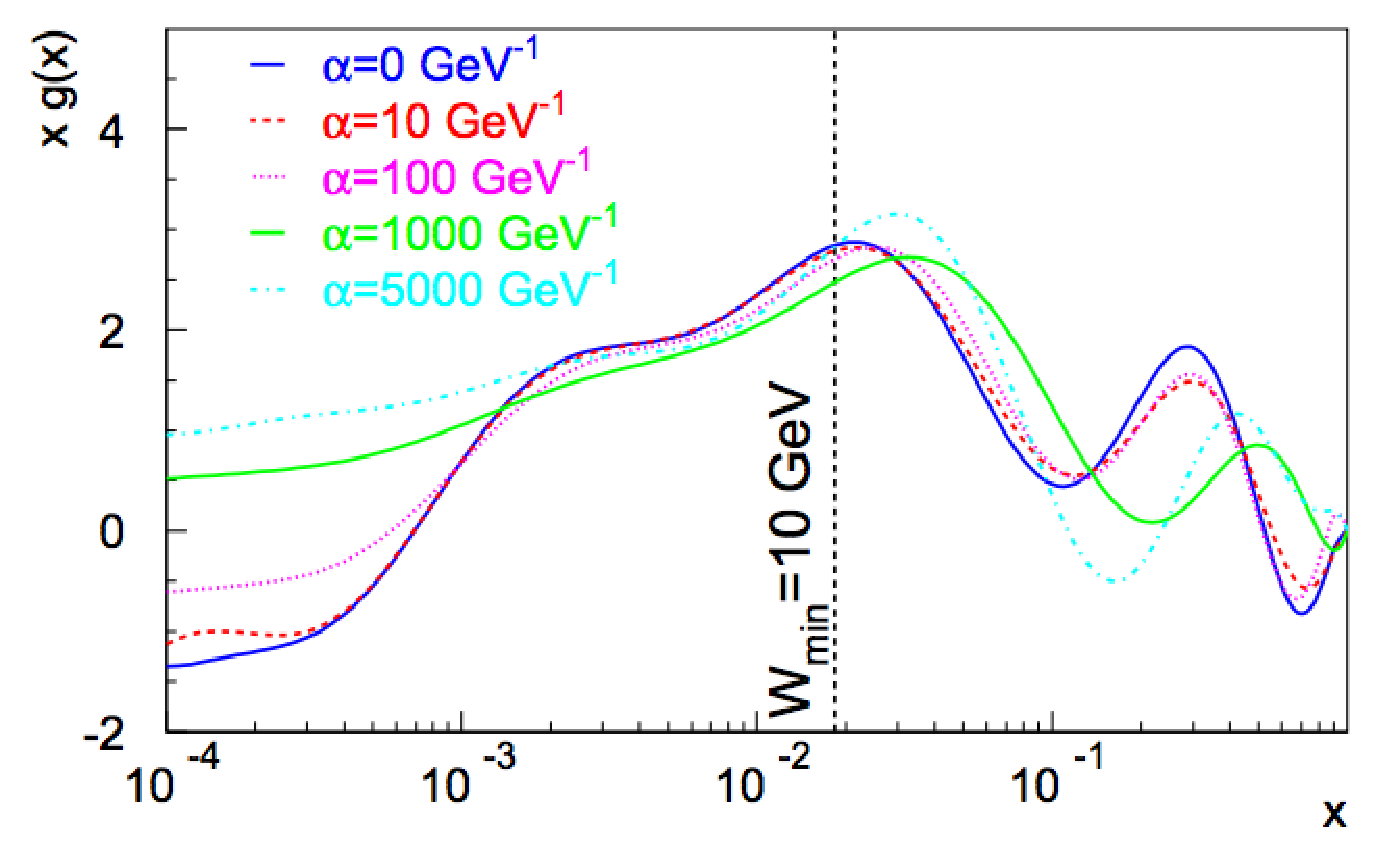
\includegraphics[width=8cm]{cheb.pdf}
 \caption{Gluon PDF at the scale of $Q^2=1.9$ GeV$^2$ for various values of the length-prior 
          weight using the Chebyshev parametrisation expanded to the 15th order.}
 \label{fig:cheb}
\end{figure}

%
\item \bf{External PDFs:} \rm 
\fitter\ also provides the possibility to access external PDF sets, which can be used to construct 
theoretical predictions for the various processes implemented in \fitter. This is possible via an 
interface to LHAPDF~\cite{lhapdf,lhapdfweb} which provides access to the global PDF sets available at LO, NLO 
or NNLO evolved either locally through the \fitter\ or taken as provided by the LHAPDF grids. 
Figure \ref{fig:pdfs} is produced with the drawing tools available in \fitter\ and illustrates 
the PDFs accessed from LHAPDF.
\end{description}
%
\begin{figure}[!ht]
   \centering
   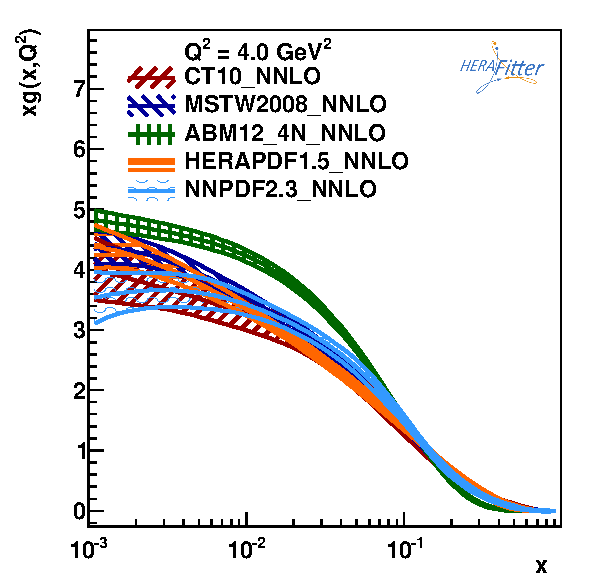
\includegraphics[width=8cm]{pdfs.pdf}
   \caption{Gluon density as extracted by various PDF groups at the scale of $Q^2=2$ GeV$^2$, plotted using the drawing tools from \fitter.} 
 \label{fig:pdfs}
\end{figure}
%
\subsection{$\chi^2$ representation}
\label{sec:chi2representation}

The PDF parameters are extracted from a $\chi^2$ minimization process. 
For experimental uncertainties there are various forms to represent the $\chi^2$ function, e.g. using a covariance matrix or representing them by nuisance parameters. 
In addition, there are various methods to deal with correlated systematic (or statistical) uncertainties (e.g. different scaling options, etc.). Here we summarise the options available in \fitter. 

\begin{description}
\item \bf {Covariance Matrix Representation:} \rm
For a data point  $\mu_i$ with a corresponding theory prediction $m_i$, the $\chi^2$ function for the case when experimental uncertainties are given as 
a covariance matrix $C_{i,j}$ over data bins $i$ and $j$, can be expressed in the following form:
%
\begin{eqnarray}
\chi^2 (m)& = & \sum_{i,j}(m_i-\mu_i)C^{-1}_{ij}(m_j-\mu_j).
\end{eqnarray}
%The $\chi^2$ function depends on the theory parameters $m^i$ 
%(denoted as the vector $\boldsymbol{m}$).
The covariance matrix can be decomposed into statistical, uncorrelated and correlated systematic contributions: 
\begin{eqnarray}
C_{ij}& = & C^{stat}_{ij}+C^{uncor}_{ij}+C^{sys}_{ij}.
\end{eqnarray}
This representation can not single out the effect of a particular
source of systematic uncertainty.

\item \bf{Nuisance Parameters Representation:} \rm
\label{sec:nuisance_representation}

%\begin{eqnarray} 
%    \chi^2\left(\boldsymbol{m},\boldsymbol{b}\right) &= &  
% \sum_i \frac{\left[m^i - \sum_j \gamma^i_j m^i b_j  - {\mu^i} \right]^2}
%{ \textstyle \delta^2_{i,{\rm stat}}\mu^i \left(m^i -  \sum_j \gamma^i_j m^i b_j\right)
%  + \left(\delta_{i,{\rm uncor}}\,  m^i\right)^2} \nonumber \\
%  &+& \sum_j b^2_j.
%\label{eq:aven}
%\end{eqnarray}
%{ \small
%\begin{equation} 
%    \chi^2\left(\boldsymbol{m},\boldsymbol{b}\right) =   
% \sum_i \frac{\left[m^i - \sum_j \gamma^i_j m^i b_j  - {\mu^i} \right]^2}
%{ \textstyle \delta^2_{i,{\rm stat}}\mu^i \left(m^i -  \sum_j \gamma^i_j m^i b_j\right)
%  + \left(\delta_{i,{\rm uncor}}\,  m^i\right)^2}+ \sum_j b^2_j.
%\label{eq:aven}
%\end{equation}}
{ \small
\begin{equation} 
    \chi^2\left(\boldsymbol{m},\boldsymbol{b}\right) =   
 \sum_i \frac{\left[ {\mu_i} - m_i \left( 1 - \sum_j \gamma^i_j b_j \right) \right]^2}
{ \textstyle \delta^2_{i,{\rm unc}}m_i^2 + \delta^2_{i,{\rm stat}}\, {\mu_i} m_i \left(1 - \sum_j \gamma^i_j b_j\right) }
  + \sum_j b^2_j.
\label{eq:aven}
\end{equation}}
%
Here ${\mu_i}$ is the  measured central value  at a point $i$ 
with  relative statistical $\delta_{i,\rm stat}$ 
and relative uncorrelated systematic uncertainty $\delta_{i,\rm unc}$.
Further, 
%$\beta_j$ denotes a nuisance parameter for
% a correlated systematic error  source of type $j$ with an uncertainty while
$\gamma^i_j$ 
quantifies the sensitivity of the
measurement ${\mu_i}$ at the point $i$ to the correlated systematic 
source $j$. The function $\chi^2$ depends in addition on
 the set of systematic nuisance parameters $b_j$.
This definition of the $\chi^2$ function assumes that
systematic uncertainties are proportional to the central prediction values
(multiplicative errors), whereas the statistical errors scale 
with the square root of the expected number of events. 
The systematic shift nuisance parameters $b_j$ as well as the PDF 
parameters are free parameters of the fit. Thus the fit determines the best fit to 
the data taking into account correlated systematic shifts of the data. 
\item  \bf{Mixed Form:} \rm
It can happen that various parts of the systematic and statistical uncertainties are stored in different forms. A situation can be envisaged when the correlated systematic experimental uncertainties are provided as nuisance parameters, but the statistical bin-to-bin correlations are given in the form of a covariance matrix. \fitter\ offers the possibility to include such information, when provided, as well as any other mixed form of treating statistical, uncorrelated and correlated systematic uncertainties. 
%In the case of off-diagonal statistical uncertainties, the $\chi^2$ function
%\begin{equation} 
%\begin{eqnarray} 
% \label{eq:chi2gen}
%    \chi^2(\boldsymbol{m},\boldsymbol{b})& = & \sum_{ij} 
%         \left ( m^i - \sum_l \gamma^i_l(m^i)b_l - \mu^i \right)  C^{-1}_{{\rm stat.}~ij}(m^i,m^j) \nonumber \\  
%    && \left(  m^j - \sum_l \gamma^j_l(m^j)b_l - \mu^j \right) +  \sum_l b^2_l.
%\end{eqnarray}
%\end{equation}
%Here the scaling properties of the correlated systematic uncertainties 
%$\Gamma^i_j$ and
%of the covariance matrix $C_{{\rm stat.}~ij}$ are expressed as a dependence
%on $m_i$ and the dependence of $\delta_{\rm stat}$ on $b_j$ is ignored.
\end{description}


\subsection{Treatment of the Experimental Uncertainties}


%Three distinct cases are implemented in \fitter\ and reviewed here:
Three distinct methods for propagating experimental uncertainties to PDFs are implemented in \fitter\ and reviewed here:
%\fitter\ provides three methods for assessing the experimental uncertainties on PDFs: 
the Hessian, Offset, and Monte Carlo method.
%Figure \ref{fig:error} illustrates the difference between the Hessian and Monte-Carlo methods both of which can be applied and plotted with \fitter.
%\begin{figure}[!ht]
%   \centering
%   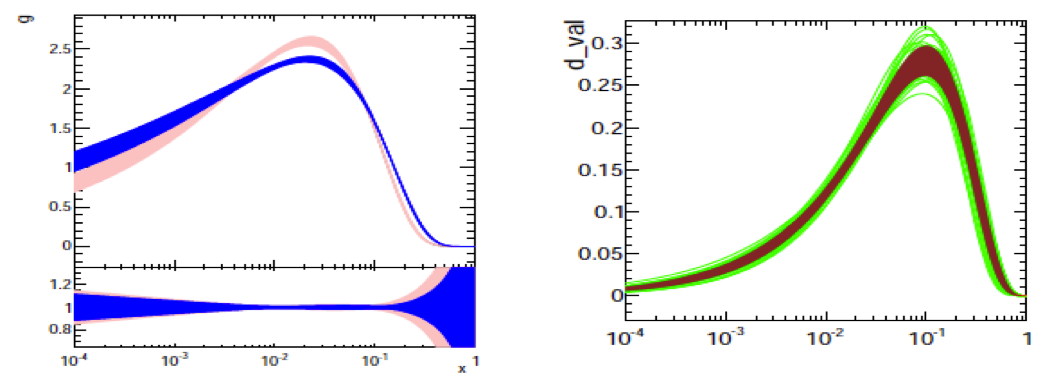
\includegraphics[width=8cm]{error.pdf}
%   \put (-206, 68) {Hessian}
%   \put (-86, 68) {Monte Carlo}
%   \caption{Differences in the experimental uncertainties on the gluon (left) and d-valence quark (right) densities extracted 
%       through different methods in \fitter: Hessian(left) versus Monte Carlo (right).} 
% \label{fig:error}
%\end{figure}
\begin{description}
\item \bf{Hessian method:} \rm
The technique developed by~\cite{Pumplin:2001ct} presents an estimate of PDF uncertainties 
reflecting the experimental precision of data used in the QCD fit by examining the behaviour 
of $\chi^2$ 
%with the nuisance parameter representation (see section~\ref{sec:nuisance_representation}) 
in the neighborhood of the minimum. 
This is known as the Hessian or error matrix method. The Hessian matrix is built by the second derivatives of $\chi^2$ at the minimum. The PDF eigenvectors are obtained through an iterative procedure used to diagonalise the Hessian matrix and rescale the eigenvectors to adapt the step sizes to their natural scale.

\item \bf{Offset  method:} \rm

Another method to propagate the correlated systematic experimental uncertainties from 
the measurements to PDFs \cite{Botje:2001fx} is Offset method.
%, which has the practical advantage that does not require the inversion of a large measurement covariance matrix.
%
It uses also the $\chi^2$ function for the central fit for which only
uncorrelated uncertainties are taken into account to get the best PDF parameters. The goodness of fit can no longer be judged from the $\chi^2$ since correlated uncertainties are ignored. 
%
The correlated systematic uncertainties of the data are then used to estimate 
the errors on the PDF parameters as follows.
The cross section is varied by one sigma shift from the central value 
for each systematic source and the fit is performed. 
%in turn the value of the cross section is offset 
This is done for both positive and negative one sigma shifts. 
After this has been done for all sources the 
resulting deviations of each of these fits from the central PDF parameters are added in quadrature. 

In most cases, the uncertainties estimated through the offset method are larger than 
those from the Hessian method, as the offset method does not use the information on correlated systematic uncertainties optimally.

\item \bf{Monte Carlo method:} \rm
The PDF uncertainties can be estimated using a Monte Carlo technique \cite{Giele:1998gw, mcmethod2}.
The method consists in preparing replicas of data sets by allowing the central values of the cross sections to 
fluctuate within their systematic and statistical uncertainties taking into account all point-to-point correlations.
The preparation of the data is repeated for a large $N$ ($>100$ times) and for each of these replicas a QCD fit is performed to 
extract the PDF set. The PDF central values and uncertainties are estimated using the mean values and standard deviations
over the replicas. 

%The MC method represents one of the main concepts of the NNPDF group.
The MC method was checked against the standard error estimation of the PDF uncertainties as used by the Hessian method. 
A good agreement was found between the methods when employing for the MC approach the assumption that uncertainties 
(statistical and systematic) follow Gaussian distribution~\cite{hera-lhc:report2009}. 
This comparison is illustrated in Fig.~\ref{fig:mchessian}. 
Similar findings were observed also in the MSTW global analysis~\cite{Watt:2012tq}. 
\begin{figure}[!ht]
 \centering
  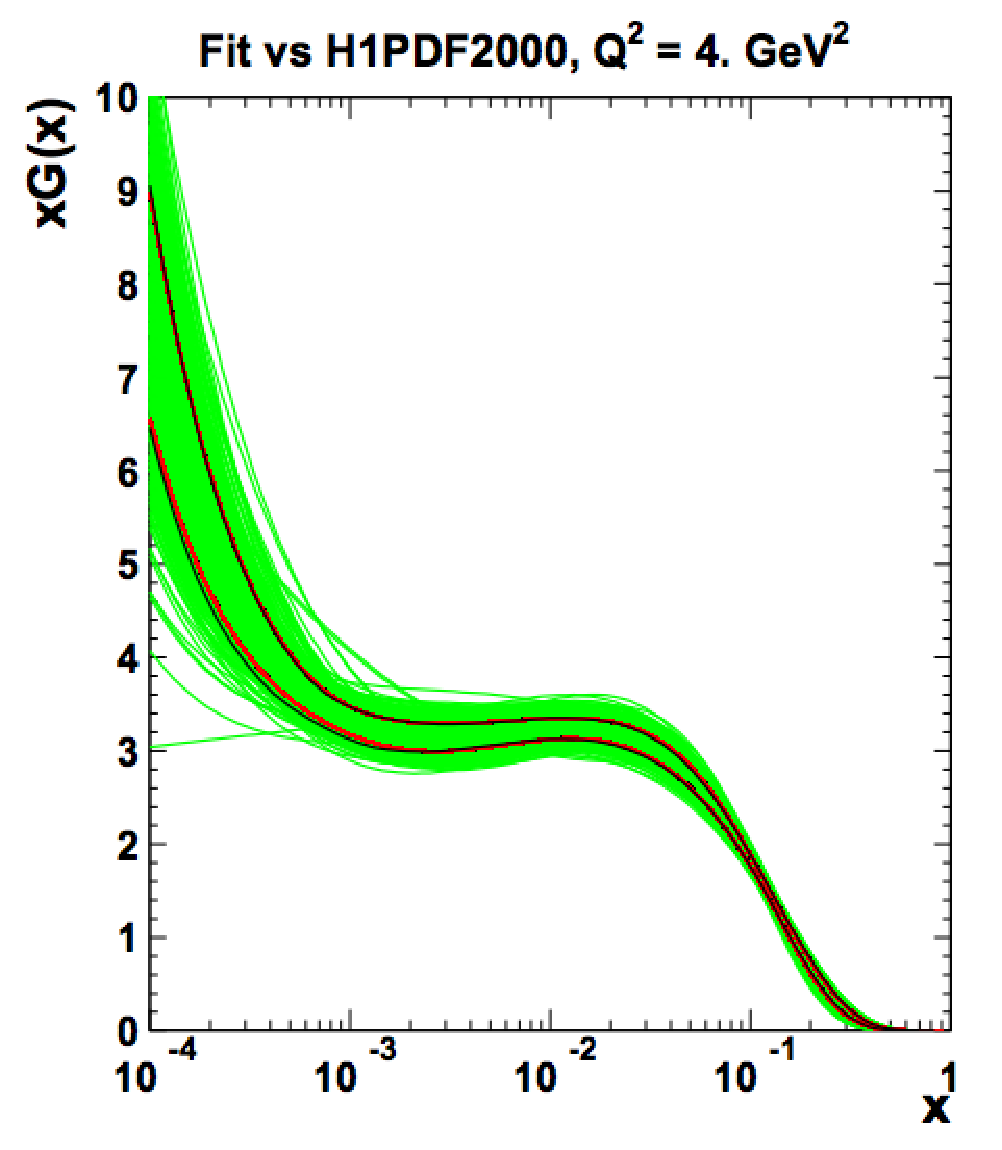
\includegraphics[width=7cm,height=7cm]{mchessian.pdf}
  \caption{Comparison between the standard error calculations as employed by the Hessian approach (black lines) 
      and the MC approach assuming Gaussian distribution for uncertainty distributions, shown here for each replica 
          (green lines) together with the evaluated standard deviation (red lines).}
  \label{fig:mchessian}        
\end{figure}
\end{description}

The usage of the nuisance parameters for the experimental uncertainty treatment in QCD fits is quite 
common and has an advantage of the flexible assessment of such uncertainties on PDFs. 
Generally, the experimental uncertainties are symmetrised when QCD fits 
are performed, however often the provided uncertainties are rather asymmetric.
\fitter\ provides the possibility to use asymmetric systematic uncertainties.
The technical implementation relies on the assumption that 
asymmetric uncertainties can be described by a parabolic function, as given below:
\begin{equation}
  f_i(b_j)=\omega^i_{j}b_j^2 + \gamma^i_{j}b_j,
\end{equation}
where the coefficients $\omega^i_{j}$, $\gamma^i_{j}$ are defined as 
up and down shifts of the cross sections to a nuisance parameter, $S_{ij}^{\pm}$, 
%{ \small
\begin{equation}
  \omega^i_{j}=\frac{1}{2}\left(S_{ij}^{-}+S_{ij}^{+}\right), \\
  \gamma^i_{j}=\frac{1}{2}\left(S_{ij}^{-}+S_{ij}^{+}\right) 
\end{equation}
%}
For this case the definition of the $\chi^2$ from Eq.~\ref{eq:aven} is extended with the parabolic approximation 
for asymmetric uncertainties, such that the expected cross section is adjusted to be
%m_i\left(1+\sum_{j}f_i(b_j)\right) = 
%{ \small
\begin{equation}
  m_i(1-\sum_j \gamma^i_{j} b_j) \to 
m_i\left(1-\sum_j b_j(\omega^i_{j}b_j + \gamma^i_{j})\right).
\end{equation}
%}
The minimisation is performed using fixed number of iterations (typically ten), with rapid convergence.





\subsection{Treatment of the Theoretical Input Parameters}

The results of a QCD fit depend not only on the input data but also on the 
input theoretical ansatz, which is also uncertain. Nowadays, modern PDF sets 
try to address the impact of the choices of theoretical parameters by providing
alternative PDFs with different choices of the mass of the charm quarks $m_c$, mass of the bottom quarks $m_b$ and the value of $\alpha_S(M_Z)$, etc. 
Another important input is the choice of the functional form for the PDFs at the starting scale and indeed the value of the starting scale itself. \fitter\ provides a platform in which such choices can readily be varied within a common framework.

\subsection{Bayesian Reweighting Techniques}

As an alternative to a complete QCD fit, the reweighting method (Bayesian Reweighting) is available in \fitter.
Because no fit is performed, the method provides a fast estimate of the impact of new data. 
The original suggestion~\cite{Giele:1998gw} was developed by the NNPDF 
collaboration \cite{Ball:2011gg,Ball:2010gb} and later extended~\cite{Watt:2012tq}
to work not only on the NNPDF replicas, but also on the eigenvectors provided by most PDF groups. 

The Bayesian Reweighting technique uses the PDF probability distributions which are modified with weights 
to account for the difference between theory predictions and new data.
In the NNPDF method the PDFs are constructed as ensembles of $N_{\rm rep}$ parton 
distribution functions and observables $\mathcal{O}(\mathrm{PDF})$ are conventionally calculated from the average
of the predictions obtained from the ensemble 
$\langle\mathcal{O}(\mathrm{PDF})\rangle =  \frac{1}{N_{\mathrm{rep}}} \sum_{k=1}^{N_{\mathrm{rep}}} \mathcal{O}(\mathrm{PDF}_k)$.
In the case of PDF uncertainties provided by standard Hessian eigenvector error sets, this can be achieved 
by creating the $k$-th random replica by introducing random fluctuations around the central PDF set.

As a next step, the initial PDF probability distributions are updated by applying weights 
$w_k$, calculated as:

\begin{equation}
 w_k = \frac{(\chi^2_k)^{\frac{1}{2} (N_{\mathrm{data}}-1) } e^{-\frac{1}{2}\chi^2_k}}{ \frac{1}{N_{\mathrm{rep}}} \sum^{N_{\mathrm{rep}}}_{k=1}(\chi^2_k)^{\frac{1}{2}(N_{\mathrm{data}}-1)} e^{-\frac{1}{2}\chi^2_k}  },
\end{equation}

where $N_{\mathrm{data}}$ is the number of new data points, $k$ denotes the specific replica for which the weight is calculated 
and $\chi^2_k$ is a difference between a given data point $y_i$ and its theoretical prediction obtained with the $k$-th PDF replica:

{\small
\begin{equation}
 \chi^2 (y,\mathrm{PDF}_k) = \sum_{i,j=1}^{N_{\mathrm{data}}} (y_i - y_i(\mathrm{PDF}_k)) \sigma^{-1}_{ij} (y_j-y_j(\mathrm{PDF}_k))  
\end{equation}
}

The new, reweighted PDFs commonly are chosen to be based upon a smaller number of PDF sets compared to the input because replicas 
that are incompatible with the data are discarded in order to create a more stream-lined PDF set.



\subsection{Performance Optimisation}

The above mentioned features make \fitter\ a powerful project that encapsulates 
state of the art developments 
%from the most up-to-date theory developments 
to debates on reaching the ultimate experimental precision. 

An important factor for a feasible QCD fit which is performed by iterative 
$\chi^2$ minimisation, is performance in terms of how long a calculation takes for each given data point.
The performance of the \fitter\  code is greatly improved with several special built-in options
including the $k-factor$ techniques (see section~\ref{sec:techniques}) and the grid techniques for the fast calculation of cross 
sections of particular processes for arbitrary sets of PDFs. There are also cache options, fast evolution kernels, and 
usage of the OpenMP (Open Multi-Processing) interface which allows
parallel applications of some of the heavy flavour scheme theory predictions in DIS. 
%{\bf please go over this, I have married two separate paragraphs that were in different places}






